The first step in TRITIUM desing was to choose the fiber length at which the signal of tritium events is optimized. On the one hand, long fibers are interesting because the efficiency of TRITIUM detector is proporcional to the fiber length, but, on the other hand, in long fibers, scintillating photons are reflected on the fiber walls more times before reaching the photosensors, that produce a deterioration in the tritium signal.

To determine the optimal length several simulations, described in section \ref{subsec:FiberLengthSimulation}, were carried out using Geant4 \cite{Geant4WebPage}, a particle and nuclear physics simulation package based on C++. It was seen that it is preferable to work with short fibers.

The fiber length for the TRITIUM prototypes developed in Valencia, was $20~\cm$, which was also the length used for most of the experiments carried out in the framework of the TRITIUM experiment. As Saint-Gobain commercial fibers are 1 meter long, an effective scintillator cutting technique had to be developed with strict requirements on the cutting quality of the fiber ends since this greatly affect the transmission of photons and, consequently, the efficiency of TRITIUM monitor. This cut must be perpendicular to the fiber and with very low uncertainty in the cutting position to achieve a good coupling of the fiber with the surface of the photosensor. It is also important that the fiber integrity be preserved, without cracks or deformations that contribute to the loss of photons.

Cutting the end faces of polymer fibers is one of current challenges. There are many different techniques such as milling, laser cutting, focused-ion-beam, blade cutting, etc. The blade cleaving technique was chosen for TRITIUM experiment because of its mechanical simplicity. %I had these references in the "Smooth end face termination of microstructured, graded-index, and step-index polymer optical fibers" paper

Many commercial devices based on blade cleaving, such as the one provided by thorlabs with a diamond tipped blade \cite{DiamondThorlabs} or others similar to guillotine designed for industrial fiber optics \cite{GuillotineIFO}, were tested in an extensive study with unsuccessful results \cite{TFGAlberto}. As it can be seen in Figures \ref{fig:BadCutsOfFibers}, Commercial techniques produce deformations, cracks and imperfections so they do not fulfill the requirements previously imposed.

\begin{figure}
\centering
    \begin{subfigure}[b]{0.5\textwidth}
    \centering
    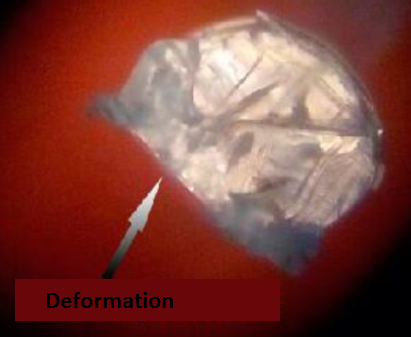
\includegraphics[width=\textwidth]{4ResearchAndDevelopments/41Fibers/DeformationFiberEnds.png}  
    \caption{Fiber end deformation.\label{subfig:FiberEndDeformation}}
    \end{subfigure}
    \hfill
    \begin{subfigure}[b]{0.45\textwidth}
    \centering
    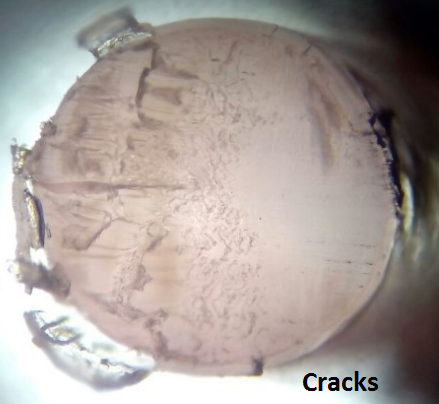
\includegraphics[width=\textwidth]{4ResearchAndDevelopments/41Fibers/CracksEndFibers.png}  
    \caption{Fiber end cracks.\label{subfig:FiberEndCracks}}
    \end{subfigure}
 \caption{Unsuccessful results of using commercial techniques to cut fibers.}
 \label{fig:BadCutsOfFibers}
\end{figure}

The microscope model PB 4161 from EUROMEX and the Digital Microscope from Jiusion were used to check the results in the fiber ends. 

Because commercial devices do not work for our scintillating fibers, a cutting device, shown in Figure \ref{fig:CuttingTRITIUMDevice}, was designed, built and tested.

\begin{figure}
\centering
    \begin{subfigure}[b]{0.4\textwidth}
    \centering
    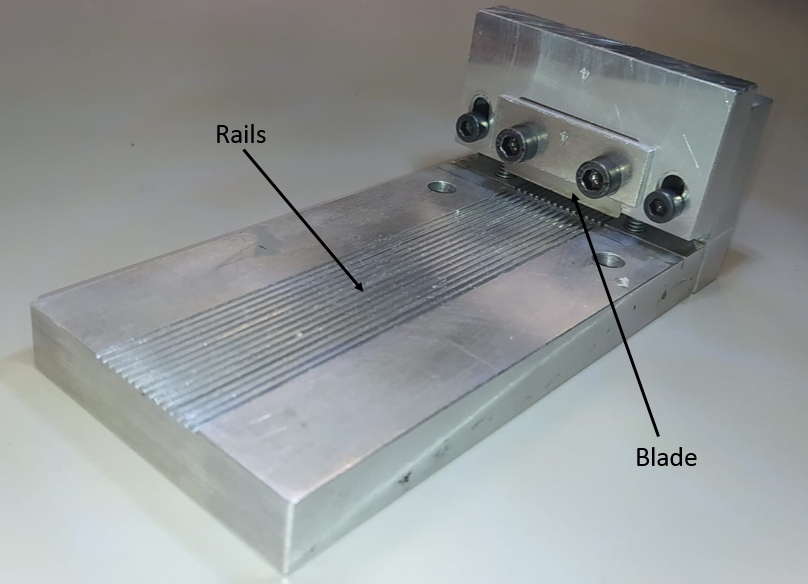
\includegraphics[width=\textwidth]{4ResearchAndDevelopments/41Fibers/CuttingDevice1.png}  
    \caption{TRITIUM Cutting device.\label{subfig:CuttingDevice1}}
    \end{subfigure}
    \hfill
    \begin{subfigure}[b]{0.55\textwidth}
    \centering
    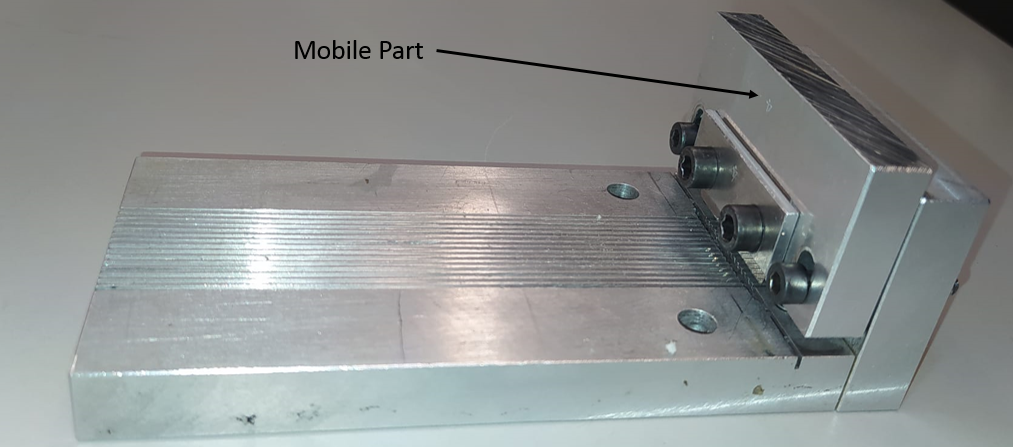
\includegraphics[width=\textwidth]{4ResearchAndDevelopments/41Fibers/CuttingDevice2.png}  
    \caption{TRITIUM Cutting device.\label{subfig:CuttingDevice2}}
    \end{subfigure}
    \hfill
    \begin{subfigure}[b]{0.6\textwidth}
    \centering
    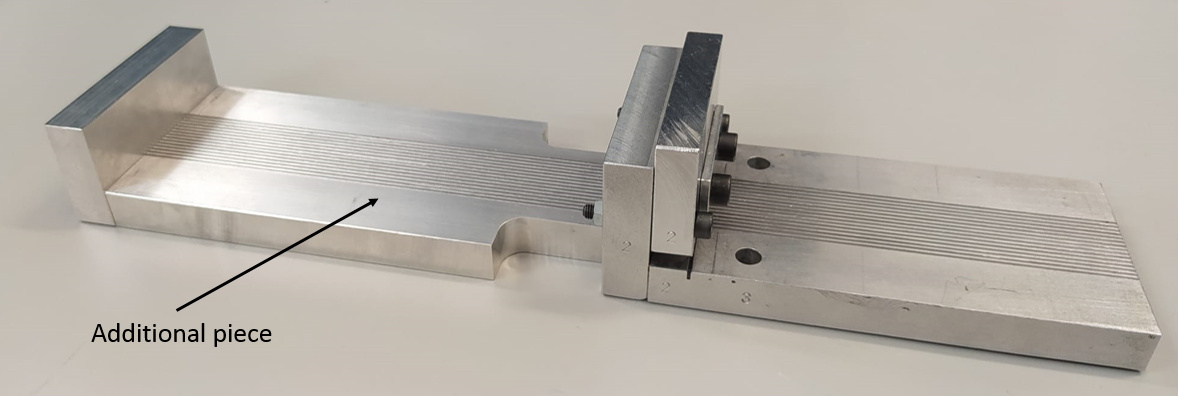
\includegraphics[width=\textwidth]{4ResearchAndDevelopments/41Fibers/AdditionalPieceCuttingDevice.png}  
    \caption{Additional piece of TRITIUM cutting device.\label{subfig:AdditionalPieceCuttingDevice}}
    \end{subfigure}
 \caption{Cutting device developed in the TRITIUM experiment and additional part to make precise measurements of fiber length.}
 \label{fig:CuttingTRITIUMDevice}
\end{figure}

This device consists of fourteen rails to which the fibers are hold and a thin blade, fixed on a mobile piece, which is used to cut them. The perpendicular cut, which is one of the requirements, can be ensured since the moving piece, to which the blades are fixed, is set perpendicular to the fibers. The blade used is a typical commercial razor blade, of $0.1~\mm$ thickness, which is the thickness that gave the best results. The blade was adjusted with $5\degree$ tilt, with respect to the horizontal axis since it was found in several studies that this helps to obtain a less aggressive and cleaner cut \cite{AngleBlade, TemperatureBlade}. As it can be seen in Figure \ref{subfig:CutFiberEnd}, with this cutting device it was obtained fiber ends without breaks or deformation.

An additional parameter that could affect the cutting quality of the fiber ends is the temperature of both, the fiber and the blade. A study was carried out in which both were subjected to different temperatures from room temperature to 110 degrees. No significant conclusions were obtained \cite{TFGAlberto}. Thus, the cutting process was carried out at room temperature to make the cutting process easier.

To set the fiber length, which is the last requirement, an additional piece was designed and built, shown in Figure \ref{subfig:AdditionalPieceCuttingDevice}. With the help of this piece an uncertainty in the fiber length of less than 1 millimeter was achieved. With the designed cutting fiber device all requirements imposed have been fulfilled, obtaining fibers with optimal light transmission.
%cutted fiber end whose quality is high enough to ensure that it will affect the transmission of light as little as possible.

The fiber end after cutting is shown in Figure \ref{subfig:CutFiberEnd}. The slightly darkened zone at the bottom of the fiber is an inavoidable effect of the cutting process and, to reduce its effect, the polishing process developed by Thorlabs was applied \cite{DiamondThorlabs}. It consists on rubbing the fibbers during two minuts with five different polishing papers, with a decreasing grain size, $30~\mu\meter$, $20~\mu\meter$, $12~\mu\meter$, $5~\mu\meter$ and $0.3~\mu\meter$, describing describing on the the paper a shape of 8 (approximately 120 movements). 

The result obtained after polishing is shown in Figure \ref{subfig:PolishFiberEnd}, where it can be noted that the darkened zone has completely disappeared and the fiber end is completely clear without any damage or imperfection. Therefore, both tasks, cutting and polishing,  are necessary.

\begin{figure}
\centering
    \begin{subfigure}[b]{0.5\textwidth}
    \centering
    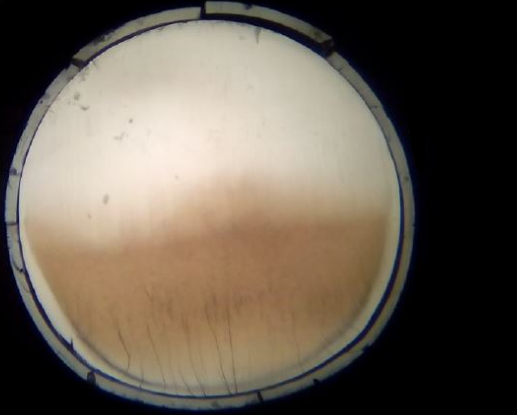
\includegraphics[width=\textwidth]{4ResearchAndDevelopments/41Fibers/CutEndFiberGood.png}  
    \caption{Fiber end after cutting with Tritium device.\label{subfig:CutFiberEnd}}
    \end{subfigure}
    \hfill
    \begin{subfigure}[b]{0.45\textwidth}
    \centering
    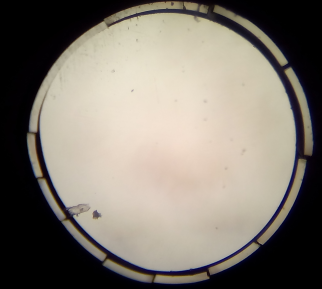
\includegraphics[width=\textwidth]{4ResearchAndDevelopments/41Fibers/CutAndPolishedFiberEnd.png}  
    \caption{Fiber end after cutting and polishing.\label{subfig:PolishFiberEnd}}
    \end{subfigure}
 \caption{Result of the polishing process. a) Fiber end after cutting b) Fiber end after cutting and polishing with Thorlabs technique.}
 \label{fig:ResultofPolishingProcess}
\end{figure}